\ifnum \Version=1
    \question[6] Use the Laplace transform and the following IVP to determine an explicit expression for $Y(s)$, which is the Laplace transform of $y(t)$. Please show your work. 
    $$9y''+ 12y' + 4y = e^{2t}\sin(3t), \ y(0) = 2, \ y'(0) = -1$$
    \ifnum \Solutions=1 {\color{DarkBlue} \\ Solution:
    \begin{align}
        \mathcal L(9y'') + \mathcal L(12y')+4Y &= \mathcal{L}(e^{2t}\sin(3t))\\ 
        9[s^2 Y - sy(0) - y'(0)]+12[sY - y(0)]+4Y &= \frac{3}{(s-2)^2+3^2} \\
        9[s^2 Y - 2s + 1] + 12[sY - 2] + 4Y &= \frac{3}{(s-2)^2+3^2} \\
        [9s^2 + 12s + 4]Y  -  18s  -  15 &= \frac{3}{(s-2)^2+3^2} 
    \end{align}
    Thus 
    \begin{align}
        Y &= \frac{18s + 15}{9s^2 + 12s + 4} +  \frac{3}{((s-2)^2+3^2)(9s^2 + 12s + 4)}
    \end{align}        
    } 
    \else 
    \vfill
    \fi         
\fi

\ifnum \Version=2
    \question[6] Use the Laplace transform and the following IVP to determine an explicit expression for $Y(s)$, which is the Laplace transform of $y(t)$. Please show your work. 
    $$y''+ 2y' - 2y = t^2, \ y(0) = 2, \ y'(0) = 1$$
    \ifnum \Solutions=1 {\color{DarkBlue} \\ Solution:
    \begin{align}
        \mathcal L[y''] + 2\mathcal L[y']-2Y &= \mathcal{L}[t^2]\\ 
        [s^2 Y - sy(0) - y'(0)]+2[sY - y(0)]-2Y &= \frac{2}{s^3} \\
        [s^2 Y + 2s - 1] + 2[sY - 2] + Y &=  \frac{2}{s^3}\\
        [s^2 + 2s -2]Y  -  2s  -  5 &=  \frac{2}{s^3}
    \end{align}
    Thus 
    \begin{align}
        Y &= \frac{2s + 5}{s^2 + 2s - 2} +  \frac{2}{s^3(s^2 + 2s - 2)}
    \end{align}        
    } 
    \else 
    \vfill
    \fi         
\fi
\ifnum \Version=3
    \question[6] Use the Laplace transform and the following IVP to determine an explicit expression for $Y(s)$, which is the Laplace transform of $y(t)$. Please show your work. 
    $$6y'' + 5y' + y = e^{-2t}, \quad y(0) = 4, \quad y'(0) = 0$$
        
    \ifnum \Solutions=1 {\color{DarkBlue} Solution:
    \begin{align}
        6\mathcal L(y'') + 5\mathcal L(y')+Y &= \mathcal L(e^{-2t})\\ 
        6[s^2 Y - sy(0) - y'(0)]+5[sY - y(0)]+Y &= 1/(s+2) \\
        6[s^2 Y - 4s] + 5[sY - 4] + Y &= 1/(s+2)\\
        [6s^2 + 5s + 1]Y  -  24s  -  20 &= 1/(s+2)
    \end{align}
    Thus 
    \begin{align}
        Y &= \frac{24s + 20}{6s^2 + 5s + 1} + \frac{1}{(s+2)(6s^2 + 5s + 1)}
    \end{align}        
    } 
    \else 
    \vfill
    \fi                

\fi


\ifnum \Version=4
    \question[6] Use the Laplace transform and the following IVP to determine an explicit expression for $Y(s)$, which is the Laplace transform of $y(t)$. Please show your work. 
    $$y''+ 12y'  = e^{2t}\cos(3t), \ y(0) = 0, \ y'(0) = 14$$
    \ifnum \Solutions=1 {\color{DarkBlue} \\ Solution:
    \begin{align}
        \mathcal L(y'') + 12\mathcal L(y') &= \mathcal{L}(e^{2t}\cos(3t))\\ 
        (s^2 Y - sy(0) - y'(0)) + 12(sY - y(0))  &= \frac{s-2}{(s-2)^2 + 3^2} \\
        (s^2 Y - 14) + 12(sY - 0)  &= \frac{s-2}{(s-2)^2 + 3^2} \\
        (s^2 + 12s )Y  &= 14 + \frac{s-2}{(s-2)^2 + 3^2} \\
        Y &= \frac{1}{s^2 + 12s } \left( 14 + \frac{s-2}{(s-2)^2 + 3^2} \right) 
    \end{align} 
    A few notes regarding the solutions below. 
    \begin{itemize}
        \item  Note that it wasn't necessary to solve the IVP so if students did solve the IVP and made mistakes along the way then there's no need to deduct points. 
        \item It wasn't necessary to determine the values of $s$ for which the transform is defined. If errors were made in working out the values of $s$ for which the transform is defined then there's no need to deduct points. 
    \end{itemize}
    } 
    \else 
    \vfill
    \fi         
\fi



\ifnum \Version=5
    \question[6] Use the Laplace transform and the following IVP to determine an explicit expression for $Y(s)$, which is the Laplace transform of $y(t)$. Please show your work. 
    $$y''+ 2y'  = e^{-3t}\sin(4t), \ y(0) = 0, \ y'(0) = 10$$
    \ifnum \Solutions=1 {\color{DarkBlue} \\ Solution:
    \begin{align}
        \mathcal L(y'') + 2\mathcal L(y') &= \mathcal{L}(e^{-3t}\sin(4t))\\ 
        (s^2 Y - sy(0) - y'(0)) + 2(sY - y(0))  &= \frac{4}{(s+3)^2 + 4^2} \\
        (s^2 Y - 10) + 2(sY - 0)  &= \frac{4}{(s+3)^2 + 4^2} \\
        (s^2 + 2s )Y  &= 10 + \frac{4}{(s+3)^2 + 4^2} \\
        Y &= \frac{1}{s^2 + 2s } \left( 10 + \frac{4}{(s+3)^2 + 4^2} \right) 
    \end{align}       
    A few notes regarding the solutions below. 
    \begin{itemize}
        \item  Note that it wasn't necessary to solve the IVP so if students did solve the IVP and made mistakes along the way then there's no need to deduct points. 
        \item It wasn't necessary to determine the values of $s$ for which the transform is defined. If errors were made in working out the values of $s$ for which the transform is defined then there's no need to deduct points. 
    \end{itemize}    
    } 
    \else 
    \vfill
    \fi         
\fi







\ifnum \Version=8
    \question[6] Use the Laplace transform and the following IVP to determine an explicit expression for $Y(s)$, which is the Laplace transform of $y(t)$. You can leave your answer in terms of $G(s)$, which is the transform of $g(t)$. Please show your work. 
    $4y''+4y'+17y=g(t), \quad y(0) = y'(0) = 0$
    \ifnum \Solutions=1 {\color{DarkBlue} Solution written below. 
        \begin{figure}[h]
        \centering
        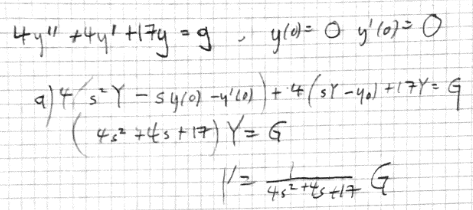
\includegraphics[width=14cm]{Images/ImgLaplaceG.png}
        \end{figure}  
    } 
    \else 
    \vfill
    \fi
\fi     